% =============================================================
% บทที่ 3 - วิธีการดำเนินงาน
% เนื้อหาแปลง/เรียบเรียงจาก Progress/Proposal ProjectNew.docx ฉบับปรับปรุงล่าสุด (หัวข้อ 5)
% แผนการดำเนินงาน (Gantt) อัปเดตตามหัวข้อ 9 ของ proposal ฉบับใหม่ (5 เดือน ปี 2569)
% ฐานข้อมูล (PostgreSQL + pgvector / Supabase) อัปเดตตาม proposal ฉบับใหม่ แทนที่ MongoDB+Chroma เดิม
% =============================================================

% -----------------------------------------------------------
\section{ขั้นตอนการดำเนินงาน}
% -----------------------------------------------------------

การดำเนินงานวิจัยนี้แบ่งออกเป็น 5 ส่วนหลัก เพื่อให้การพัฒนาแอปพลิเคชันเป็นไปอย่างมีระบบและครอบคลุมทั้งด้านเทคโนโลยี การจัดการข้อมูล การออกแบบสถาปัตยกรรมระบบ และการประเมินผลลัพธ์ โดยเนื้อหาในส่วนนี้อ้างอิงจากการออกแบบและพัฒนาต้นแบบระบบ (Prototype) ที่ดำเนินการจริงในงานวิจัย ได้แก่ เว็บแอปพลิเคชันแนะนำการท่องเที่ยวจังหวัดขอนแก่นที่ประกอบด้วยระบบ แชตบอต ให้คำแนะนำและระบบวางแผนการเดินทางที่ขับเคลื่อนด้วยโมเดลภาษาขนาดใหญ่ (LLM) ร่วมกับเทคนิค RAG

\subsection{ศึกษาปัญหาและรวบรวมความต้องการ}

\subsubsection{การศึกษาวรรณกรรมและทฤษฎีที่เกี่ยวข้อง}

ขั้นตอนนี้มีวัตถุประสงค์เพื่อรวบรวมและวิเคราะห์แนวคิด เทคนิค และเครื่องมือที่ทันสมัยในการพัฒนาระบบแนะนำการท่องเที่ยว (Tourism Recommender Systems: TRS) และระบบอัจฉริยะ เพื่อใช้เป็นกรอบแนวคิดในการออกแบบระบบ

\begin{enumerate}[label=(\arabic*),leftmargin=0pt,itemindent=\dimexpr\parindent+\parenlabelwidth+1em\relax,align=right,labelwidth=\parenlabelwidth,labelsep=1em]
\item การศึกษาระบบแนะนำการท่องเที่ยวและการวางแผนการเดินทาง: ศึกษาแนวคิดพื้นฐานของระบบ TRS และวิวัฒนาการไปสู่ระบบที่พิจารณาหลายภาคส่วน (Multistakeholder Recommendation) โดยเฉพาะแนวโน้มการบูรณาการปัจจัยด้านความยั่งยืน (Sustainability) เข้าไปในการวางแผนการเดินทาง ซึ่งครอบคลุมทั้งมิติเศรษฐกิจ สังคม และสิ่งแวดล้อม แนวคิดนี้ถูกนำมาใช้เป็นกรอบอ้างอิงในการออกแบบเกณฑ์การให้คำแนะนำของระบบ กล่าวคือ การจัดลำดับและคัดเลือกสถานที่ในแผนการเดินทางของงานวิจัยนี้พิจารณาปัจจัยด้านงบประมาณ ระยะเวลา ความสนใจของผู้ใช้ และระยะทาง/เวลาการเดินทางระหว่างสถานที่ร่วมกัน โดยยังไม่ได้นำปัจจัยด้านผลกระทบสิ่งแวดล้อมเชิงปริมาณ (เช่น Carbon Footprint) มาใช้ในการคำนวณโดยตรงในต้นแบบปัจจุบัน ซึ่งจะกล่าวถึงในฐานะแนวทางการต่อยอดงานวิจัยในอนาคต
\item การศึกษาเทคโนโลยีปัญญาประดิษฐ์สำหรับการประมวลผลภาษาธรรมชาติ: ศึกษานวัตกรรมที่ใช้โมเดลภาษาขนาดใหญ่ (LLMs) และการประมวลผลภาษาธรรมชาติ (NLP) สำหรับการสร้างคำแนะนำและการตอบโต้กับผู้ใช้งาน โดยเน้นที่สถาปัตยกรรม RAG ซึ่งเป็นแนวทางที่มีประสิทธิภาพในการจัดการข้อมูลการท่องเที่ยวที่มีการเปลี่ยนแปลงอยู่เสมอ (Dynamic Data) โดยไม่จำเป็นต้องปรับจูนโมเดล LLM (Fine-tuning) ซ้ำทุกครั้งที่ข้อมูลเปลี่ยนแปลง แนวคิดนี้ถูกนำไปประยุกต์ใช้จริงในทั้งส่วนของระบบ แชตบอต และระบบวางแผนการเดินทางของงานวิจัยนี้
\item การศึกษาสถาปัตยกรรมระบบสำหรับแอปพลิเคชัน AI: ศึกษาแนวทางการออกแบบระบบแบบแยกส่วนบริการ (Service-Oriented / Microservices Architecture) ซึ่งช่วยให้แต่ละองค์ประกอบของระบบสามารถพัฒนา ทดสอบ และปรับขนาด (Scale) ได้อย่างเป็นอิสระต่อกัน อันเหมาะสมกับแอปพลิเคชัน AI ที่มีภาระการประมวลผลแตกต่างกันในแต่ละส่วน (เช่น การประมวลผลภาษาธรรมชาติที่ใช้ทรัพยากรสูงกว่าการให้บริการข้อมูลทั่วไป) แนวคิดนี้ถูกนำมาใช้เป็นหลักในการออกแบบระบบจริงของงานวิจัย
\end{enumerate}

\subsubsection{การเก็บรวบรวมและเตรียมข้อมูล}

การเตรียมข้อมูลถือเป็นรากฐานสำคัญในการสร้างระบบอัจฉริยะที่แม่นยำและน่าเชื่อถือ

\begin{enumerate}[label=(\arabic*),leftmargin=0pt,itemindent=\dimexpr\parindent+\parenlabelwidth+1em\relax,align=right,labelwidth=\parenlabelwidth,labelsep=1em]
\item การรวบรวมข้อมูลแหล่งท่องเที่ยวและกิจกรรม: ข้อมูลหลักของระบบรวบรวมจาก Google Places API (New) ครอบคลุมข้อมูลสถานที่ท่องเที่ยว โรงแรม/ที่พัก และร้านอาหารในพื้นที่จังหวัดขอนแก่น โดยข้อมูลที่ดึงมาประกอบด้วยชื่อสถานที่ ประเภท/แท็ก พิกัดภูมิศาสตร์ คะแนนรีวิว ระดับราคา เวลาทำการ (รวมช่วงเวลาเปิด--ปิดแบบละเอียดรายวัน) และสถานะทางธุรกิจ (Business Status) การนำเข้าข้อมูลในระยะต้นแบบนี้ดำเนินการผ่านสคริปต์ดึงและนำเข้าข้อมูลแบบครั้งเดียว มิใช่การซิงค์ข้อมูลแบบเรียลไทม์ โดยผู้ดูแลระบบสามารถเพิ่มหรือแก้ไขข้อมูลสถานที่ กิจกรรม และฐานความรู้เพิ่มเติมภายหลังได้ผ่านหน้าจอผู้ดูแลระบบ (Admin Dashboard) ที่พัฒนาขึ้นเป็นส่วนหนึ่งของระบบ
\item การเตรียมและจัดเก็บข้อมูล:
\begin{enumerate}[label=(2.\arabic*),leftmargin=0pt,itemindent=\dimexpr\parindent+\parenlabelwidth+1em+\subParenLabelWidth+1em\relax,align=right,labelwidth=\subParenLabelWidth,labelsep=1em]
\item การทำความสะอาดและจัดรูปแบบข้อมูล (Data Preprocessing): ข้อมูลดิบที่รวบรวมมาจะถูกนำมาแปลงให้อยู่ในรูปแบบมาตรฐานของระบบ (Normalizing) เช่น การรวมประเภทสถานที่ย่อยจาก Google ให้อยู่ในหมวดหมู่ภาษาไทยที่ระบบใช้งาน (เช่น ร้านอาหาร คาเฟ่ วัด พิพิธภัณฑ์ สวนสาธารณะ ตลาด ที่พัก) และการตรวจสอบความสมบูรณ์ของข้อมูลก่อนบันทึกลงฐานข้อมูล
\item การแบ่งส่วนข้อมูลและการสร้างเวกเตอร์ (Chunking and Vector Embeddings): สำหรับการใช้งานร่วมกับ RAG ข้อมูลแต่ละรายการ (สถานที่ กิจกรรม และเนื้อหาในฐานความรู้) จะถูกแปลงเป็นเวกเตอร์ฝังตัว (Vector Embeddings) ด้วยโมเดล paraphrase-multilingual-MiniLM-L12-v2 (384 มิติ) ซึ่งประมวลผลบนเครื่องคอมพิวเตอร์ในเครื่อง (Local Inference) ผ่านไลบรารี sentence-transformers โดยจะมีการคำนวณเวกเตอร์ใหม่ทุกครั้งที่มีการนำเข้าหรือแก้ไขข้อมูล
\item การจัดเก็บในฐานข้อมูลเวกเตอร์: เวกเตอร์ที่สร้างขึ้นจะถูกจัดเก็บไว้ในฐานข้อมูล PostgreSQL ตัวเดียวกับที่จัดเก็บข้อมูลหลักของระบบ โดยอาศัยส่วนขยาย pgvector ในการจัดเก็บและคำนวณค่าความคล้ายคลึงเชิงมุม (Cosine Similarity) การเลือกใช้ฐานข้อมูลเดียวกันแทนการติดตั้งฐานข้อมูลเวกเตอร์แยกต่างหาก ช่วยลดความซับซ้อนของระบบในระยะต้นแบบ และยังคงประสิทธิภาพการค้นคืนที่เพียงพอสำหรับขนาดข้อมูลของกรณีศึกษานี้
\end{enumerate}
\end{enumerate}

\subsection{วิเคราะห์และออกแบบระบบ}

การพัฒนาระบบแบ่งออกเป็น 3 องค์ประกอบที่พัฒนาและรันแยกจากกัน (Independent Services) ได้แก่ ส่วนเว็บแอปพลิเคชัน (Frontend) ส่วนบริการข้อมูลหลัก (Backend API) และส่วนบริการปัญญาประดิษฐ์ (AI Service) ซึ่งครอบคลุมทั้งระบบ แชตบอต และระบบวางแผนการเดินทาง

\begin{enumerate}[label=(\arabic*),leftmargin=0pt,itemindent=\dimexpr\parindent+\parenlabelwidth+1em\relax,align=right,labelwidth=\parenlabelwidth,labelsep=1em]
\item การออกแบบสถาปัตยกรรมระบบ: ระบบที่พัฒนาในงานวิจัยนี้ใช้แนวทางสถาปัตยกรรมไมโครเซอร์วิส (Microservices Architecture) ซึ่งประกอบด้วย 3 บริการหลักที่เป็นอิสระต่อกัน คือ Frontend Service, Backend API Service และ AI Service สื่อสารระหว่างกันผ่าน RESTful API เท่านั้น โดยรายละเอียดเทคโนโลยีและหน้าที่ของแต่ละบริการอธิบายไว้ในบทที่ 4 หัวข้อสถาปัตยกรรมของระบบ

\begin{figure}[H]
\centering
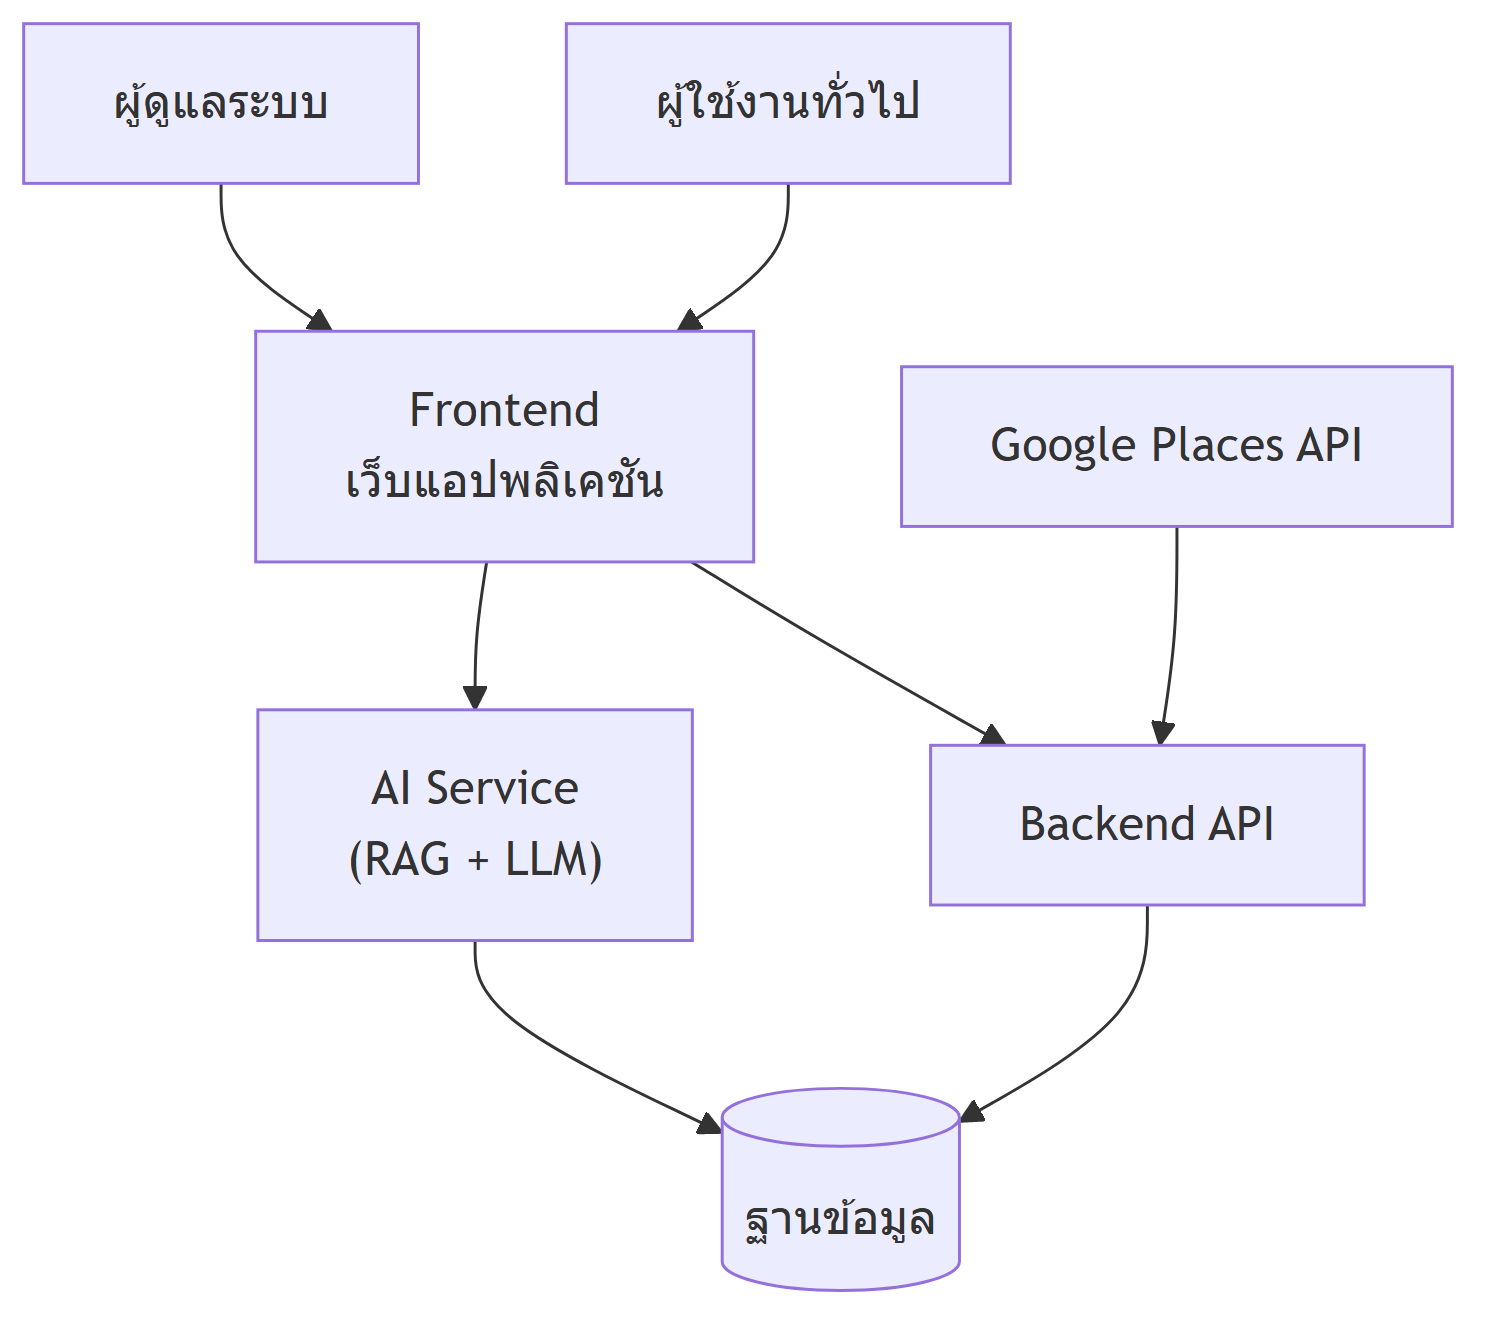
\includegraphics[width=0.75\textwidth,height=9.5cm,keepaspectratio]{images/image12.png}
\caption{แผนภาพสถาปัตยกรรมระบบของงานวิจัย}
\end{figure}

\item การออกแบบ UX/UI ของเว็บแอปพลิเคชัน: กำหนดโฟลว์การใช้งาน (User Flow) ตั้งแต่การเข้าสู่ระบบ การป้อนความต้องการท่องเที่ยว ไปจนถึงการรับแผนการเดินทางที่ระบบสร้างให้ ออกแบบหน้าจอสำคัญ เช่น หน้าแรก หน้ารายละเอียดสถานที่/กิจกรรม หน้าแบบฟอร์มวางแผนทริป และหน้าแสดงผลแผนการเดินทาง โดยยึดหลักการออกแบบที่มีผู้ใช้เป็นศูนย์กลาง
\end{enumerate}

\subsection{พัฒนาระบบ}

\begin{enumerate}[label=(\arabic*),leftmargin=0pt,itemindent=\dimexpr\parindent+\parenlabelwidth+1em\relax,align=right,labelwidth=\parenlabelwidth,labelsep=1em]
\item การพัฒนาระบบวางแผนการเดินทาง (Trip Planning): ระบบวางแผนการเดินทางใช้กลไก LLM ร่วมกับ RAG และชั้นการคำนวณเชิงกำหนดแน่นอน (Deterministic Computation Layer) ทำงานร่วมกันเป็นกลไกหลักในการสร้างแผนการเดินทาง โดยมีขั้นตอนดังนี้

\begin{figure}[H]
\centering
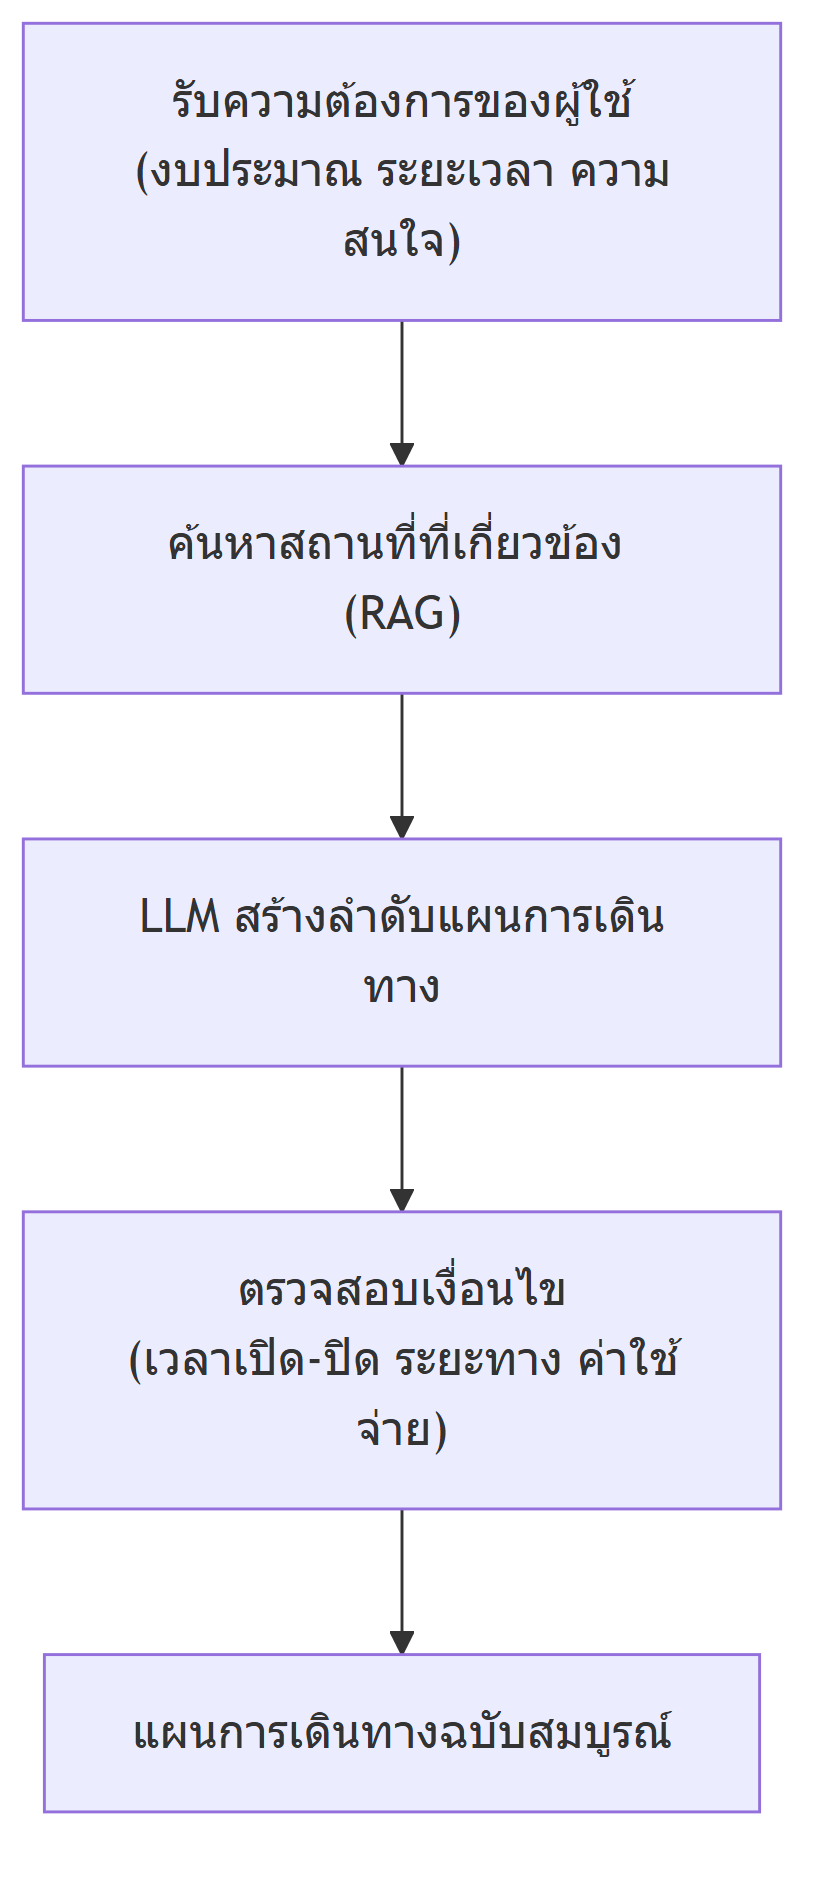
\includegraphics[width=0.75\textwidth,height=9.5cm,keepaspectratio]{images/image13.png}
\caption{แผนภาพขั้นตอนการทำงานของระบบวางแผนการเดินทาง}
\end{figure}

ระบบประมวลผลตามลำดับ 4 ขั้นตอนหลัก ได้แก่ การทำความเข้าใจความต้องการของผู้ใช้ (Query Understanding) การค้นคืนสถานที่ผู้สมัครด้วยเทคนิค RAG แบบผสม (Candidate Retrieval) การให้ LLM สังเคราะห์แผนการเดินทางโดยอ้างอิงเฉพาะสถานที่ผู้สมัครที่ให้ไป (Prompt Construction \& Generation) และการตรวจสอบความถูกต้องของแผนด้วยกลไกคำนวณซ้ำแบบกำหนดแน่นอนที่ทำงานอิสระจาก LLM (Guardrails / Constraint Verification)

\item การพัฒนาระบบ แชตบอต และระบบแนะนำ (Chatbot and Recommendation System):

\begin{figure}[H]
\centering
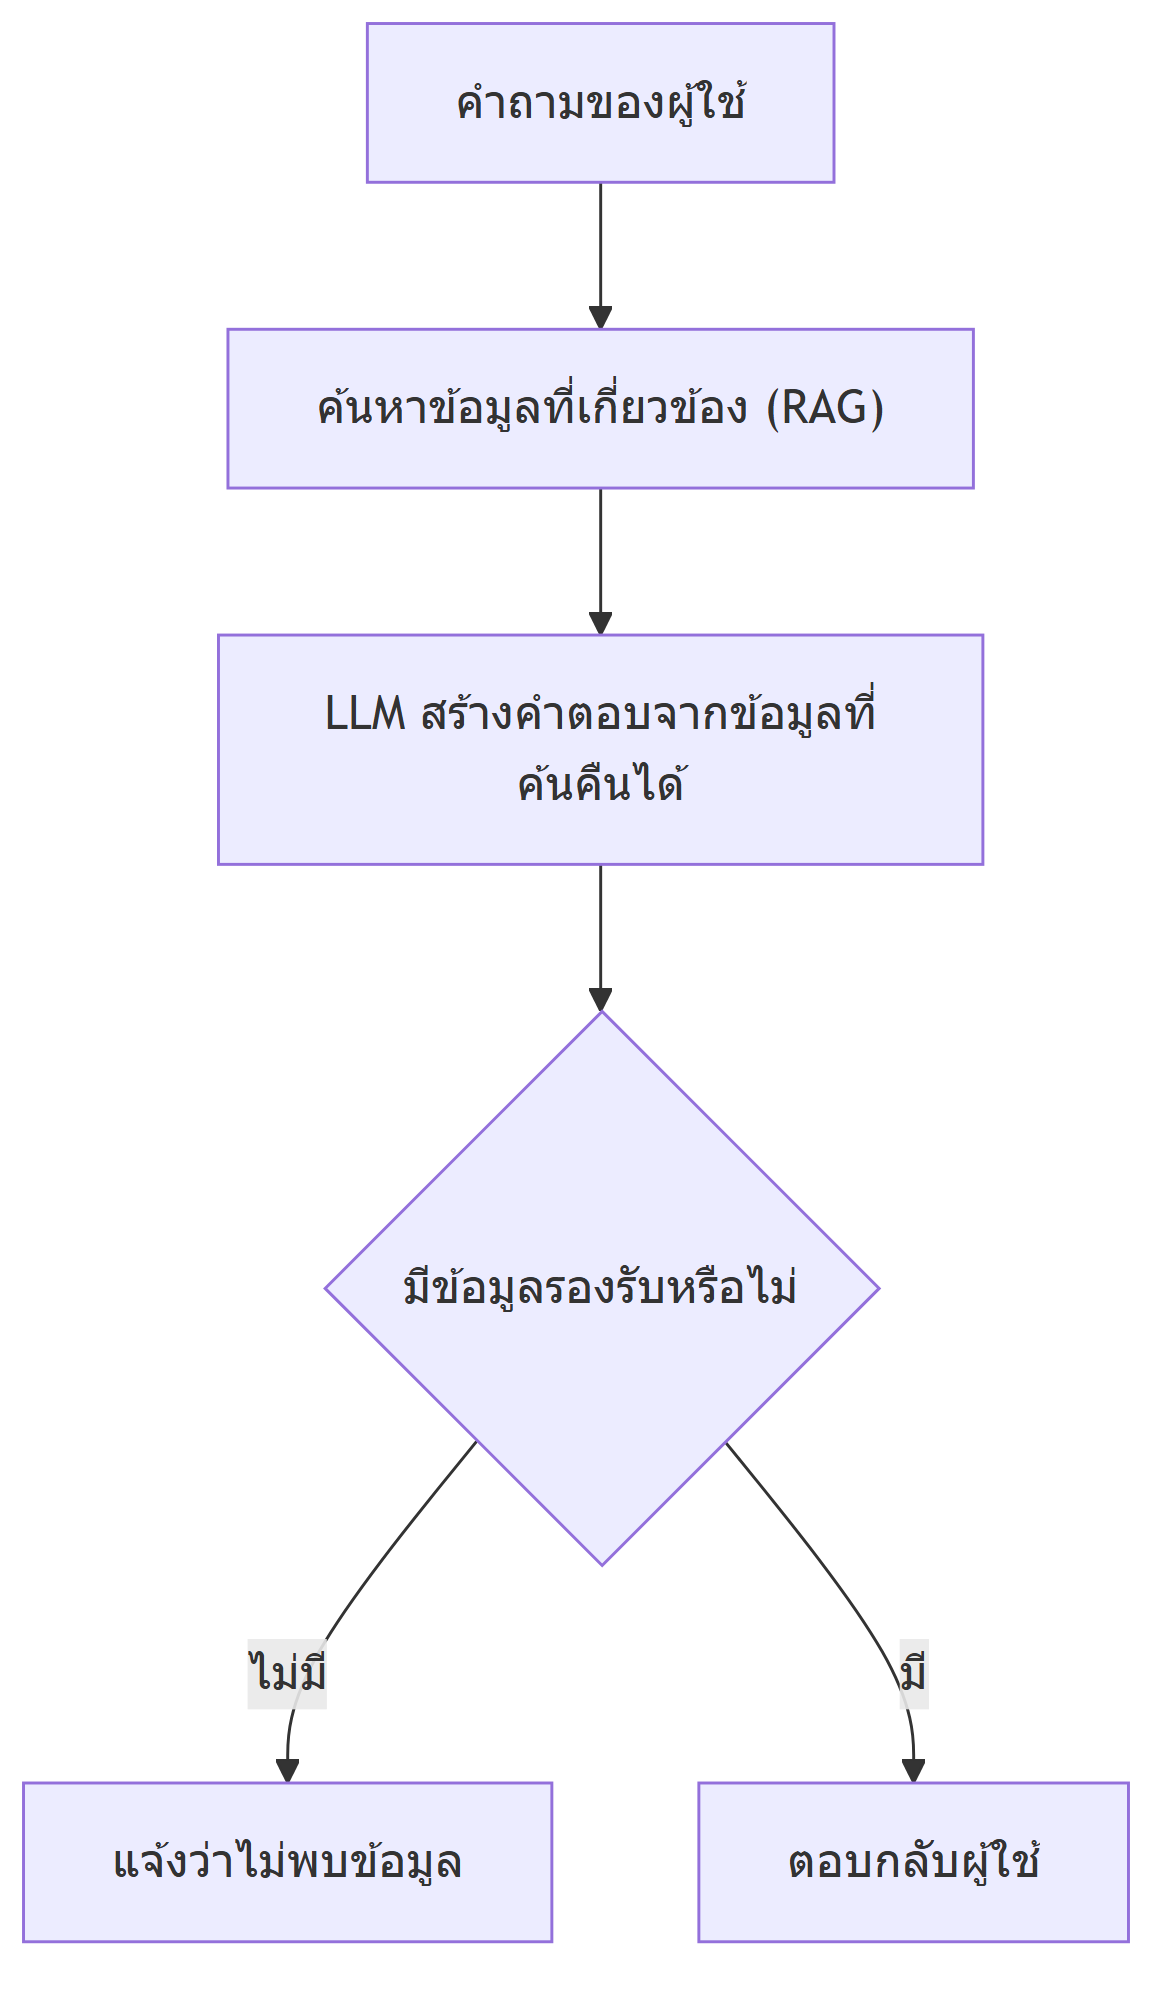
\includegraphics[width=0.75\textwidth,height=9.5cm,keepaspectratio]{images/image14.png}
\caption{แผนภาพขั้นตอนการทำงานของระบบ แชตบอต และระบบแนะนำ}
\end{figure}

ระบบประมวลผลคำถามของผู้ใช้ผ่าน 3 ขั้นตอนหลัก ได้แก่ การเขียนคำถามใหม่และค้นคืนข้อมูลที่เกี่ยวข้องด้วยเทคนิค RAG แบบผสม (Information Retrieval) การให้ LLM สังเคราะห์คำตอบแบบทยอยแสดงผลพร้อมกลไกป้องกันการตอบข้อมูลที่ไม่มีหลักฐานรองรับ (Response Generation with Hallucination Guard) และการจัดอันดับสถานที่แนะนำจากผลการค้นคืน (Recommendation)

\item การพัฒนา Frontend: พัฒนาด้วยเฟรมเวิร์ก React ร่วมกับเครื่องมือ Vite เพื่อสร้างส่วนติดต่อผู้ใช้ที่โต้ตอบได้และรองรับการใช้งานข้ามอุปกรณ์ (Responsive Web Design) ทั้งบน Desktop, Tablet และ Mobile
\item การพัฒนา Backend และการเชื่อมต่อกับบริการต่าง ๆ: ออกแบบ RESTful API สำหรับดึงข้อมูลจากบริการวางแผนการเดินทาง ระบบแนะนำ และข้อมูลกิจกรรม/สถานที่ พัฒนาหน้าจอสำหรับผู้ดูแลระบบ (Admin Dashboard) เพื่อจัดการข้อมูลสถานที่ กิจกรรม ฐานความรู้ และรหัส QR สำหรับระบบสะสมคะแนน
\item การทดสอบด้านการใช้งาน (Usability Testing): ทดสอบกับกลุ่มผู้ใช้เป้าหมาย (นักศึกษา/นักท่องเที่ยวในจังหวัดขอนแก่น) โดยใช้เกณฑ์ประเมินด้านความง่ายในการใช้งาน ความพึงพอใจและความเข้าใจในการนำเสนอข้อมูล
\end{enumerate}

\subsection{ทดสอบและประเมินผล}

\begin{enumerate}[label=(\arabic*),leftmargin=0pt,itemindent=\dimexpr\parindent+\parenlabelwidth+1em\relax,align=right,labelwidth=\parenlabelwidth,labelsep=1em]
\item การทดสอบประสิทธิภาพของระบบวางแผนการเดินทาง: วัดผลลัพธ์ของระบบวางแผนการเดินทางด้วยตัวชี้วัดหลายด้าน (Performance Metrics) ได้แก่ เวลาตอบสนอง (Response Time) คือระยะเวลารวมที่ระบบใช้ตั้งแต่รับคำขอจนถึงส่งแผนการเดินทางสำเร็จให้ผู้ใช้ แยกพิจารณาเป็นเวลาในขั้นตอนการค้นคืนข้อมูล (Retrieval) และขั้นตอนการสังเคราะห์แผนของ LLM ความแม่นยำในการตอบสนองความต้องการของผู้ใช้ (Accuracy in Meeting User Preferences) คือสัดส่วนของความต้องการที่ผู้ใช้ระบุ (เช่น งบประมาณ สถานที่ที่ต้องไปแน่นอน ความสนใจ) ที่ปรากฏอยู่ในแผนการเดินทางที่ระบบสร้างจริง; และตัวชี้วัด Pass Rate ที่ปรับจากกรอบแนวคิด TravelPlanner ให้สอดคล้องกับขอบเขตของระบบ แบ่งเป็น 3 ตัวชี้วัดเชิงปริมาณ (\%) คือ Environment Constraint Pass Rate (อัตราส่วนสถานที่/ร้านอาหารในแผนการเดินทางที่มีอยู่จริงในฐานข้อมูลของระบบ ซึ่งเป็นผลจากกลไก Grounded Generation โดยตรง จึงใช้ยืนยันความถูกต้องของกลไกป้องกัน Hallucination), Commonsense Constraint Pass Rate (อัตราส่วนแผนงานที่มีความสมเหตุสมผลเชิงเวลาและการเดินทาง เช่น ไม่จัดกิจกรรมซ้อนเวลา ไม่ไปสถานที่ที่ปิดทำการ ระยะเวลาเดินทางระหว่างจุดสอดคล้องกับระยะทางจริง) และ Hard Constraint Pass Rate (อัตราส่วนแผนงานที่บรรลุเงื่อนไขที่ผู้ใช้กำหนดครบถ้วน ทั้งงบประมาณ ระยะเวลา และสถานที่ที่ต้องไปแน่นอน)

\item การประเมินผลโมเดล RAG/แชตบอต: ประเมินความเกี่ยวข้องของคำตอบ (Answer Relevance) ว่าคำตอบที่สร้างโดย LLM ตอบคำถามของผู้ใช้ได้ดีเพียงใด โดยใช้ LLM อีกตัวหนึ่งที่แยกอิสระจากโมเดลที่ใช้งานจริงในระบบเป็นผู้ประเมิน (LLM-as-a-Judge) ให้คะแนนในระดับ 0--100 เพื่อลดความลำเอียงจากการใช้โมเดลเดียวกันทั้งสร้างคำตอบและประเมินผล; ประเมินความน่าเชื่อถือ (Faithfulness) โดยนับจำนวนคำตอบที่หลุดออกนอกบริบทที่ค้นคืนได้ (Out-of-Context) ซึ่งบ่งชี้ถึงการเกิด Hallucination ของโมเดล โดยเปรียบเทียบผลก่อนและหลังการเปิดใช้งานกลไกแท็กกำกับคำตอบเพื่อยืนยันประสิทธิภาพของกลไกดังกล่าว; และประเมิน Context Recall / Precision ของขั้นตอนการค้นคืนข้อมูล (Retrieval) ว่าสามารถดึงข้อมูลสถานที่/ฐานความรู้ที่เกี่ยวข้องกับคำถามจริงออกมาได้ครบถ้วนและแม่นยำเพียงใด โดยเปรียบเทียบผลระหว่างการค้นคืนด้วยความคล้ายคลึงเชิงเวกเตอร์อย่างเดียวกับการค้นคืนแบบผสม (Hybrid Search) ที่ระบบใช้งานจริง เพื่อยืนยันความคุ้มค่าของการออกแบบดังกล่าว

\item การประเมินความพึงพอใจของผู้ใช้: ใช้แบบสอบถามเพื่อประเมินความรู้สึกและทัศนคติของผู้ใช้เมื่อมีปฏิสัมพันธ์กับระบบ AI โดยวัดความพึงพอใจโดยรวม ความรู้สึกด้านบวกหรือด้านลบ และการยอมรับทางเทคโนโลยี สำหรับ แชตบอต จะประเมินความพึงพอใจของผู้ใช้ ร่วมกับค่า Precision, Recall และ F-score ของความสามารถในการตอบคำถามให้ตรงประเด็นเพิ่มเติม
\end{enumerate}

\subsection{ปรับปรุงและสรุปผล}

\begin{enumerate}[label=(\arabic*),leftmargin=0pt,itemindent=\dimexpr\parindent+\parenlabelwidth+1em\relax,align=right,labelwidth=\parenlabelwidth,labelsep=1em]
\item การวิเคราะห์ผลลัพธ์ของโมเดล: เปรียบเทียบผลการประเมินที่ได้จากหัวข้อการทดสอบและประเมินผล โดยเน้นการวิเคราะห์เชิงลึก 2 ส่วน คือ Trip Planning วิเคราะห์ว่าการผสานกลไก LLM เข้ากับชั้นการคำนวณเชิงกำหนดแน่นอน (Deterministic Backstop) ภายใต้สถาปัตยกรรมแบบแยกส่วนบริการสามารถยกระดับคุณภาพของแผนการเดินทาง (Itinerary Quality) ได้อย่างมีประสิทธิภาพตามเป้าหมายที่ตั้งไว้หรือไม่ เมื่อเทียบกับแนวทางที่ใช้ LLM สร้างแผนโดยไม่มีชั้นตรวจสอบเพิ่มเติม; และ แชตบอต วิเคราะห์ว่ากลไก RAG ร่วมกับการค้นคืนแบบผสม (Hybrid Search) ช่วยให้ระบบให้คำแนะนำที่ถูกต้องและมีความเกี่ยวข้องของคำตอบสูงขึ้นโดยไม่เพิ่มอัตราการเกิด Hallucination หรือไม่ เมื่อเทียบกับแนวทางค้นคืนด้วยความคล้ายคลึงเชิงเวกเตอร์เพียงอย่างเดียว

\item การวิเคราะห์เชิงพฤติกรรมและการยอมรับของผู้ใช้: วิเคราะห์ข้อมูลความพึงพอใจของผู้ใช้ โดยพิจารณาว่าผู้ใช้รับรู้ถึงประโยชน์หลักของการใช้ AI อย่างไร (เช่น การเข้าถึงข้อมูลที่รวดเร็วขึ้น การได้รับแผนการเดินทางที่ตรงความต้องการโดยไม่ต้องค้นหาข้อมูลเอง เวลาที่ใช้ในการวางแผนสั้นลง) และระบุข้อกังวลหลักของผู้ใช้ (เช่น ความถูกต้องของข้อมูลที่ AI ให้ ความเป็นส่วนตัวและความปลอดภัยของข้อมูล การพึ่งพาเทคโนโลยีสูง) ซึ่งข้อมูลเหล่านี้สามารถนำไปสู่การปรับปรุงความโปร่งใสของระบบ (เช่น การแสดงแหล่งที่มาของคำแนะนำ) และการสร้างความเชื่อมั่นในระบบ

\item การสรุปผลและข้อเสนอแนะ: สรุปผลลัพธ์หลักที่แสดงให้เห็นถึงความสำเร็จของการบูรณาการ LLM และเทคนิค RAG เข้ากับสถาปัตยกรรมแบบแยกส่วนบริการในการวางแผนการเดินทางและการแนะนำการท่องเที่ยว พร้อมระบุข้อจำกัดที่พบในงานวิจัย ได้แก่ (1) ปัญหา Cold-start สำหรับผู้ใช้ใหม่ที่ยังไม่มีประวัติความสนใจ (2) ขนาดชุดข้อมูลที่จำกัดเฉพาะพื้นที่จังหวัดขอนแก่น (3) ระบบยืนยันตัวตนที่ยังอยู่ในรูปแบบจำลองและยังไม่รองรับการใช้งานจริงเต็มรูปแบบ จากข้อจำกัดดังกล่าว งานวิจัยนี้เสนอแนวทางสำหรับการพัฒนาต่อยอดในอนาคต ได้แก่ การขยายขอบเขตให้ครอบคลุมตัวชี้วัดด้านความยั่งยืนเชิงปริมาณที่ยังไม่ได้นำมาใช้ในต้นแบบปัจจุบัน (เช่น Carbon Footprint จากการเดินทาง และผลกระทบทางเศรษฐกิจต่อผู้ประกอบการท้องถิ่น) การเสริมสถาปัตยกรรมด้วย API Gateway และ Message Broker เพื่อรองรับการขยายตัวของระบบ การพัฒนาระบบยืนยันตัวตนให้สมบูรณ์ และการพัฒนาไปสู่ระบบแนะนำแบบสนทนาที่ซับซ้อนยิ่งขึ้น (Conversational Recommender System) ที่สามารถปรับแผนการเดินทางแบบโต้ตอบกับผู้ใช้ได้แบบต่อเนื่อง
\end{enumerate}

% -----------------------------------------------------------
\section{เครื่องมือที่ใช้ในการดำเนินงาน}
% -----------------------------------------------------------


% TODO: ยังไม่มีรายละเอียดสเปกฮาร์ดแวร์ที่ใช้จริงในเอกสารต้นฉบับ (Proposal / Research Me) -- กรอกเพิ่มเติมภายหลัง

\subsection{ซอฟต์แวร์}

เครื่องมือด้านซอฟต์แวร์ที่ใช้ในการพัฒนาโครงงานแสดงดังตารางที่ \ref{tab:software}

\begin{table}[H]
\centering
\caption{รายการซอฟต์แวร์ที่ใช้ในการพัฒนา}
\label{tab:software}
\begin{tabular}{|c|p{4.3cm}|p{6.5cm}|}
\hline
\textbf{ลำดับ} & \textbf{ซอฟต์แวร์} & \textbf{วัตถุประสงค์} \\
\hline
1 & React (Vite) & พัฒนา Frontend Service (Web) \\ \hline
2 & Node.js (Express) & พัฒนา Backend API Service หลัก \\ \hline
3 & Python (FastAPI) & พัฒนา AI Service สำหรับระบบ แชตบอต และระบบวางแผนการเดินทาง (RAG) \\ \hline
4 & PostgreSQL (Supabase) + pgvector & จัดเก็บข้อมูลหลักของระบบและเวกเตอร์ฝังตัว (Vector Embeddings) สำหรับ RAG ในฐานข้อมูลเดียวกัน \\ \hline
5 & sentence-transformers (paraphrase-multilingual-MiniLM-L12-v2) & สร้างเวกเตอร์ฝังตัวแบบประมวลผลในเครื่อง (Local Inference) \\ \hline
6 & gemini-2.5-flash (ผ่าน OpenAI-compatible API) & โมเดลภาษาขนาดใหญ่ (LLM) สำหรับแชตบอตและการวางแผนทริป \\ \hline
7 & Google Places API & ดึงข้อมูลตั้งต้น (Data Seeding) ของสถานที่ท่องเที่ยว \\
\hline
\end{tabular}
\end{table}

% -----------------------------------------------------------
\section{แผนการดำเนินงาน}
% -----------------------------------------------------------

แผนการดำเนินงานตลอดระยะเวลาโครงงานแสดงดังตารางที่ \ref{tab:gantt} โดยแรเงาเข้ม (\colorbox{gray!60}{\phantom{xx}}) หมายถึงช่วงเวลาที่ดำเนินการเสร็จสิ้นแล้วจริง และแรเงาอ่อน (\colorbox{gray!25}{\phantom{xx}}) หมายถึงช่วงเวลาที่กำลังดำเนินการอยู่ ณ ขณะจัดทำรายงานฉบับนี้ (เดือนที่ 8) ส่วนช่องว่างหมายถึงยังไม่ถึงกำหนดหรือยังไม่เริ่มดำเนินการ

\begin{table}[H]
\centering
\caption{แผนการดำเนินงาน (Gantt Chart)}
\label{tab:gantt}
\begin{tabular}{|p{5.5cm}|c|c|c|c|c|}
\hline
 & \multicolumn{5}{c|}{ปี 2569} \\
\hline
การดำเนินงาน & 6 & 7 & 8 & 9 & 10 \\
\hline
1. การศึกษาวรรณกรรมและทฤษฎีที่เกี่ยวข้อง
 & \cellcolor{gray!60} & & & & \\
\hline
2. การเก็บรวบรวมและเตรียมข้อมูล
 & \cellcolor{gray!60} & \cellcolor{gray!60} & & & \\
\hline
3. การออกแบบและพัฒนาระบบ
 & & \cellcolor{gray!60} & \cellcolor{gray!60} & & \\
\hline
4. การทดสอบและประเมินผลระบบ
 & & & \cellcolor{gray!25} & \cellcolor{gray!25} & \\
\hline
5. การวิเคราะห์และสรุปผล
 & & & & & \\
\hline
\end{tabular}
\end{table}

ณ ช่วงเวลาจัดทำรายงานฉบับนี้ (เดือนที่ 8 ปี 2569) การดำเนินงานเป็นไปตามแผนที่วางไว้ กล่าวคือ ขั้นตอนที่ 1--3 (การศึกษาวรรณกรรม การเก็บรวบรวมข้อมูล และการออกแบบ/พัฒนาระบบ) เสร็จสิ้นแล้ว โดยระบบทั้งสามส่วน (Frontend, Backend, AI Service) เชื่อมต่อและทำงานร่วมกันได้จริงแบบครบวงจรตามที่อธิบายไว้ในบทที่ 4 และ 5 ส่วนขั้นตอนที่ 4 (การทดสอบและประเมินผลระบบ) อยู่ระหว่างดำเนินการ โดยได้จัดทำชุดทดสอบอัตโนมัติครอบคลุมกลไก LLM-as-a-Judge และระบบวางแผนการเดินทางบางส่วนแล้ว แต่การทดสอบเชิงประเมินผลเต็มรูปแบบตามตัวชี้วัดในหัวข้อ 3.4 (Pass Rate, Answer Relevance, Faithfulness ฯลฯ) และการทดสอบกับผู้ใช้งานจริง (UAT) ยังไม่ได้ดำเนินการ จึงยังไม่สามารถเริ่มขั้นตอนที่ 5 (การวิเคราะห์และสรุปผล) ได้อย่างสมบูรณ์ ทั้งนี้คาดว่าจะยังคงดำเนินการตามกรอบเวลาเดิมได้ในเดือนที่ 9--10 ต่อไป